\chapter{Architecture}
In this thesis, we design and implement a data-driven learning interest recommendation system and integrate with current MOOC platform.
In this chapter, we  will introduce the system architecture and user data flow.
Moreover, we will also introduce the website MVC design and the website models.

\section{Layer Structure Overview}
This system can be divided into three parts: user interface, web server and data-service server. (see Figure \ref{fig:layer-overview}).
User interface is focus on precessing user's interaction and contains two parts, website view and data analysis view.
Website view is contents peovided by web server, which contains all MOOC learning and management features for users to interact with,
Data analysis view, on the other hand, is the content of analyzed result based on events triggered by users, which will presented by visualizing the processed data.
Web server is mainly handling requests from user interface.
Data-service is a API server collects user interface's activitiy datas and analyze it afterward, and furthermote send back the analyzed data result back to user interface whenever user send a specific request to data-service server.

\begin{figure}[H]
    \centering
    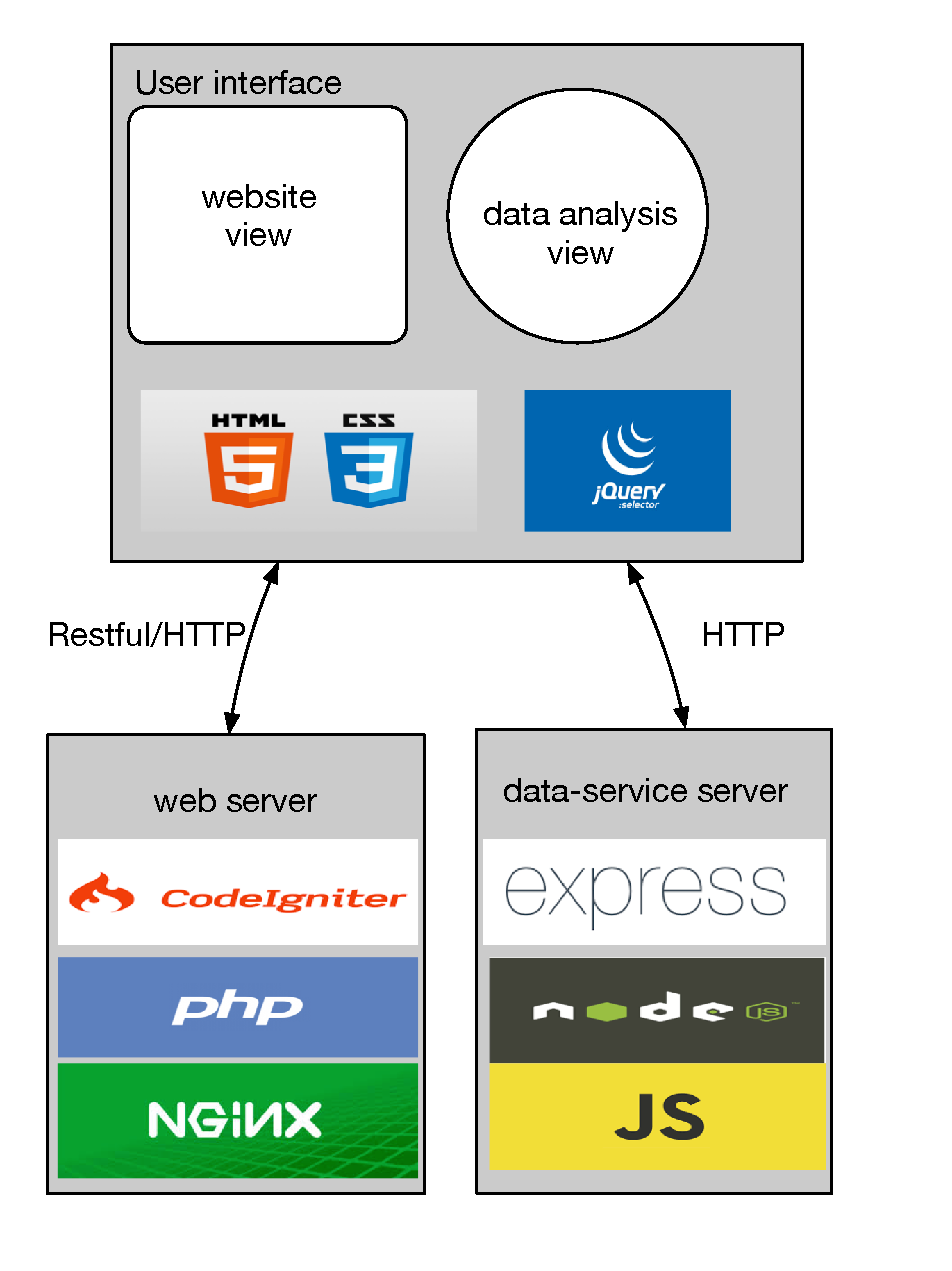
\includegraphics[width = 0.8\textwidth]{fig/layer-structure-overview.eps}
    \caption{layer structure overview}
    \label{fig:layer-overview}
\end{figure}

\section{System Architecture}
Figure \ref{fig:sys-arch} illustrates

\begin{figure}[H]
    \centering
    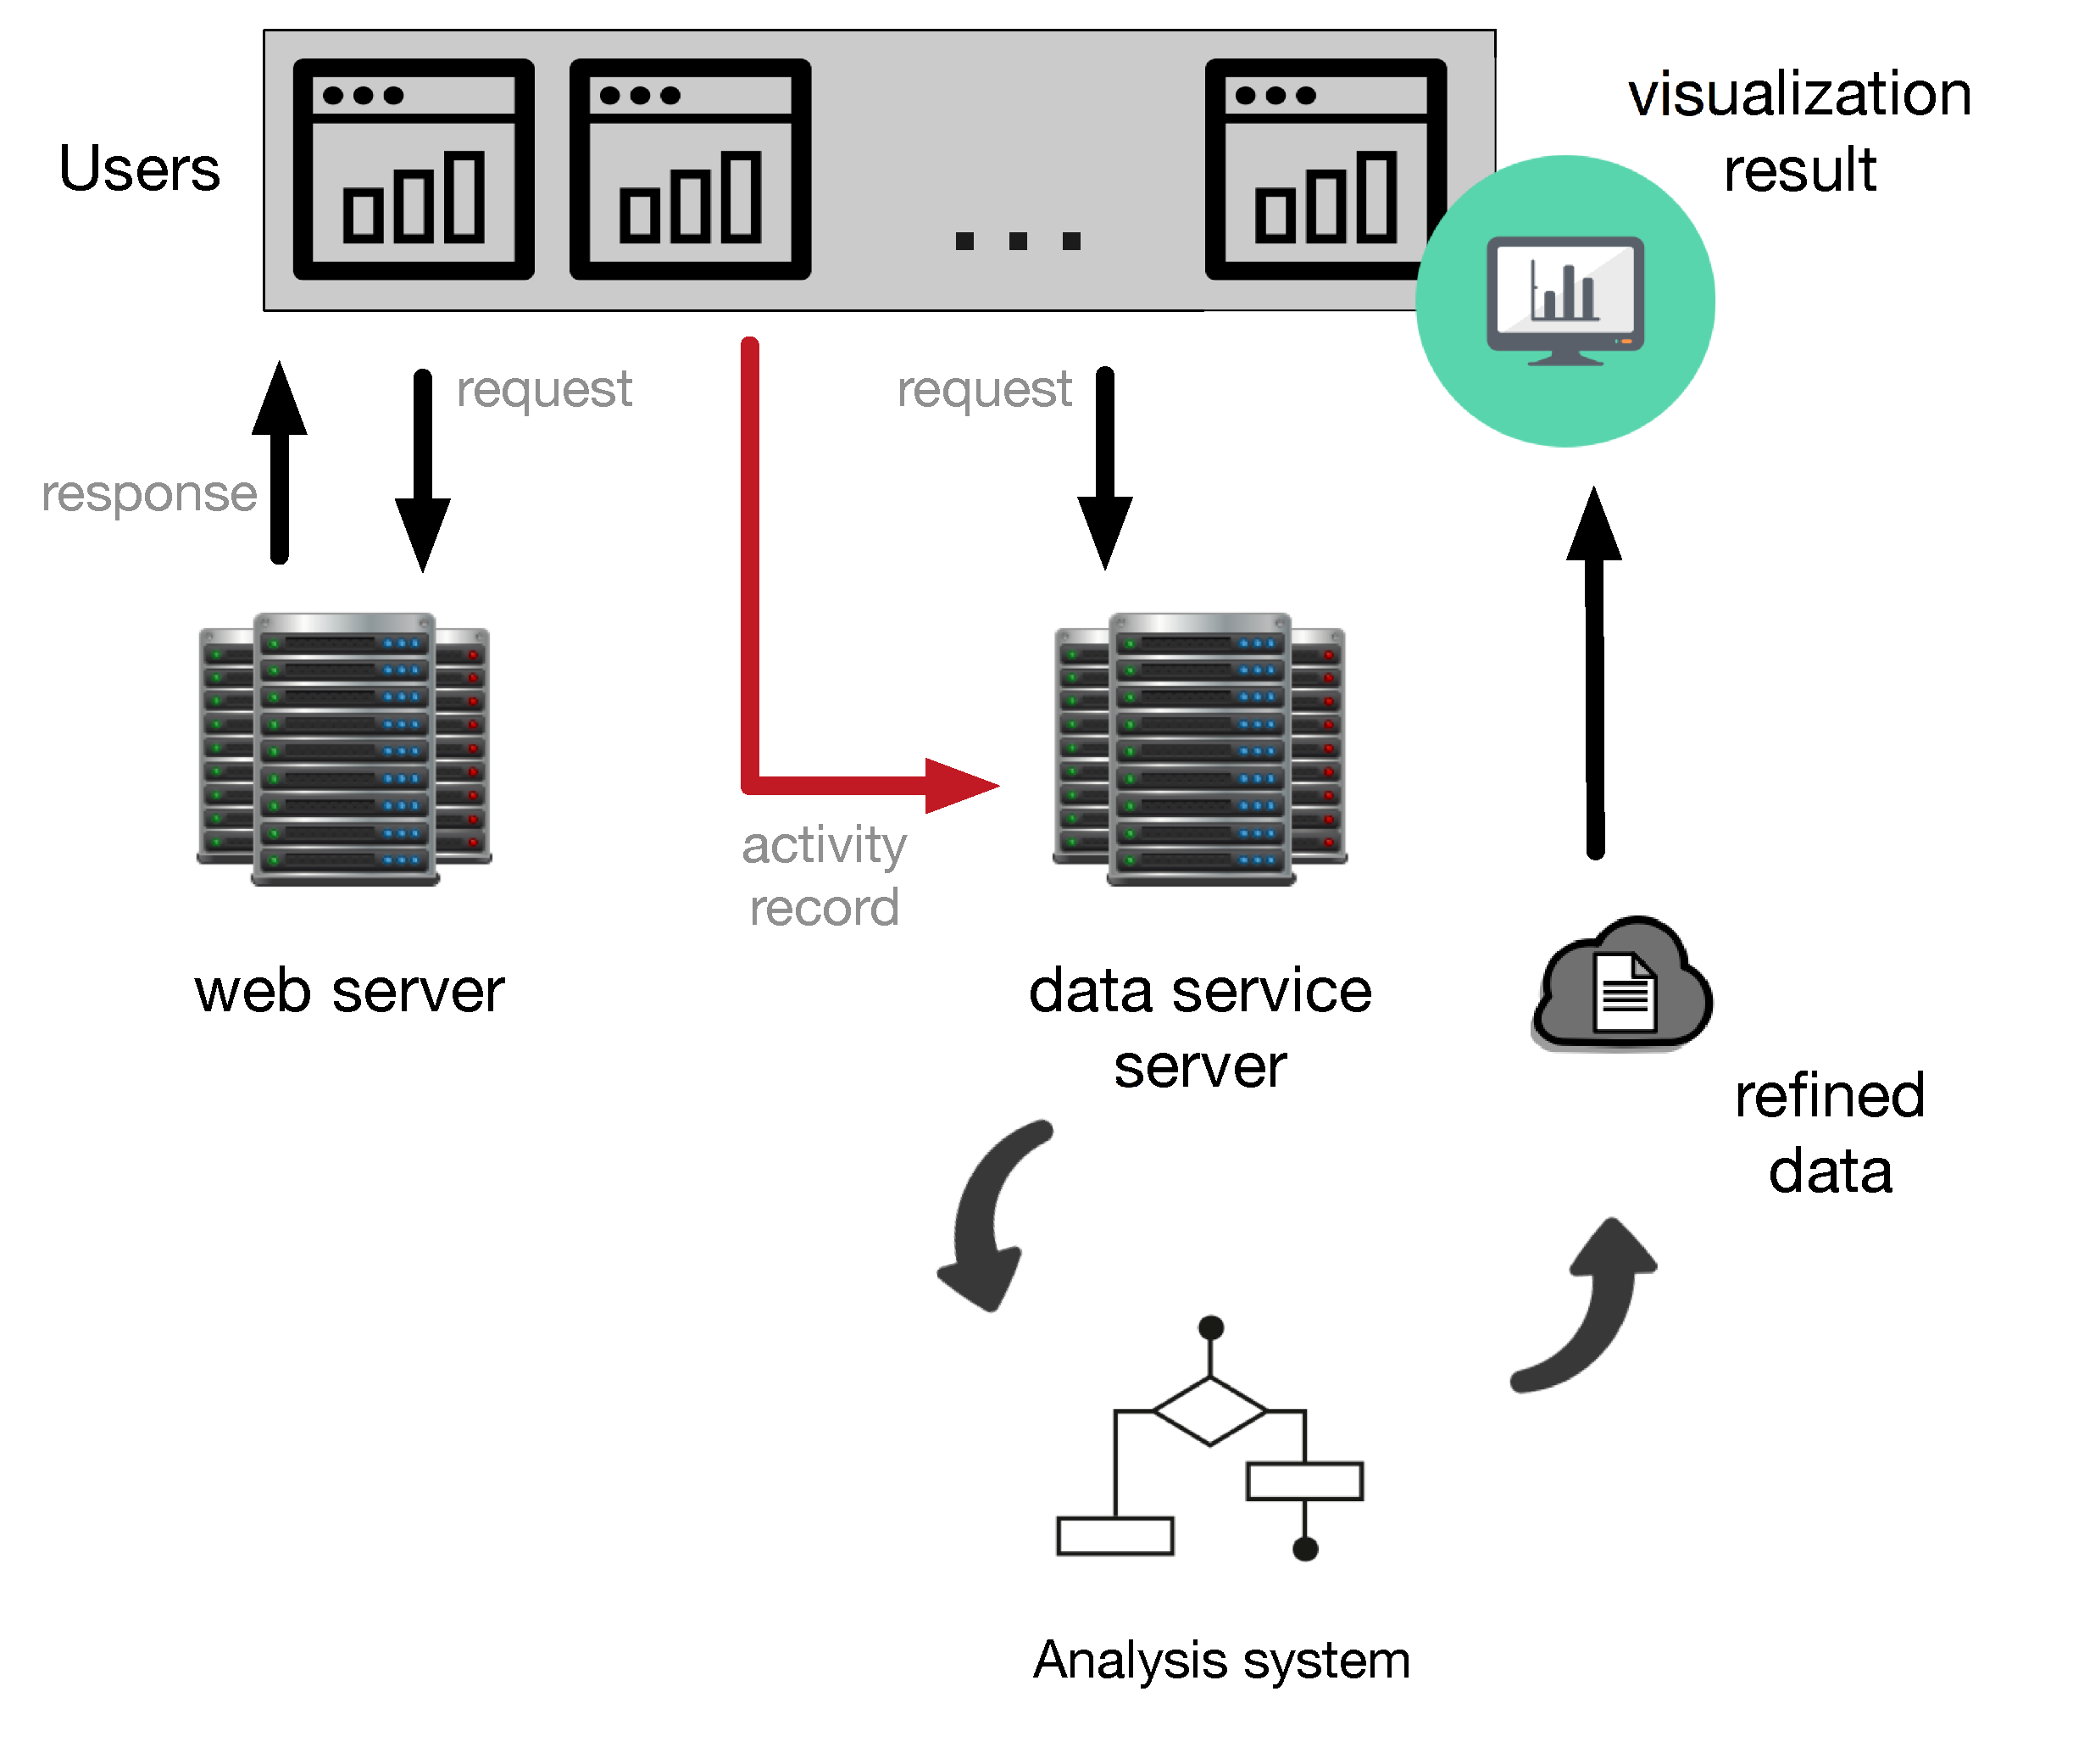
\includegraphics[width = 0.8\textwidth]{fig/system-architecture-outline.eps}
    \caption{layer structure overview}
    \label{fig:sys-arch}
\end{figure}
